\documentclass[aspectratio=169]{beamer}
\usetheme{Madrid}
\usecolortheme{default}

\usepackage[T1]{fontenc}
\usepackage[utf8]{inputenc}
\usepackage[english]{babel}
\usepackage{booktabs}
\usepackage{array}
\usepackage{graphicx}
\usepackage{tikz}
\usepackage{qrcode}
\usetikzlibrary{arrows.meta,positioning,fit,calc}

\title{PushWorld: Optimizing Learned Search}
\subtitle{Inference-time optimizations for a frozen transformer policy}
\author{Evgeny Ivankin, Adam Suliman}
\date{}

\newcommand{\metric}[2]{\textbf{#1}\\{\scriptsize #2}}

\begin{document}

\begin{frame}
  \titlepage
\end{frame}

\begin{frame}{Training setup and evaluation target}
  \small
  \begin{columns}[T]
    \column{0.52\textwidth}
    \textbf{Policy training}
    \begin{itemize}
      \item Expert traces generated by the official C++ N+RGD planner.
      \item Imitation learning on roughly half of all Level-0 puzzle families.
      \item No Level-1 training signal in the checkpoint used for these search experiments.
      \item Model weights are fixed during all optimizations in this presentation.
    \end{itemize}

    \column{0.48\textwidth}
    \textbf{Evaluation}
    \begin{itemize}
      \item 68 original Level-1 puzzles.
      \item Maximum 100 actions per puzzle.
      \item Metrics: solved puzzles, wall-clock time, solves/minute, model evaluations.
      \item Same checkpoint, different inference/search strategy.
    \end{itemize}
  \end{columns}
\end{frame}

\begin{frame}{Model architecture}
  \small
  \begin{center}
  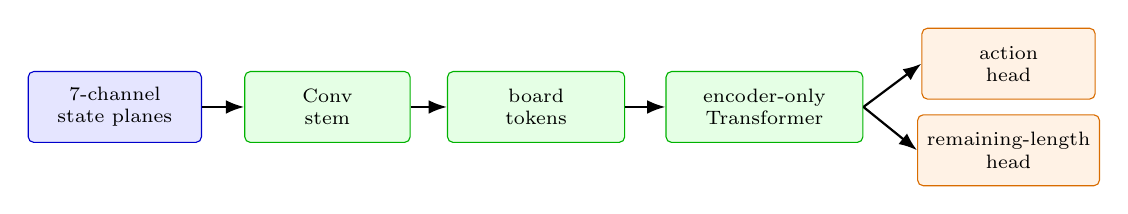
\begin{tikzpicture}[>=Latex]
    \node[draw=blue!80!black, fill=blue!10, rounded corners=2pt, align=center, minimum width=2.2cm, minimum height=0.9cm, font=\scriptsize] (planes) at (0,0) {7-channel\\state planes};
    \node[draw=green!70!black, fill=green!10, rounded corners=2pt, align=center, minimum width=2.1cm, minimum height=0.9cm, font=\scriptsize] (conv) at (2.7,0) {Conv\\stem};
    \node[draw=green!70!black, fill=green!10, rounded corners=2pt, align=center, minimum width=2.25cm, minimum height=0.9cm, font=\scriptsize] (tokens) at (5.35,0) {board\\tokens};
    \node[draw=green!70!black, fill=green!10, rounded corners=2pt, align=center, minimum width=2.5cm, minimum height=0.9cm, font=\scriptsize] (tr) at (8.25,0) {encoder-only\\Transformer};
    \node[draw=orange!85!black, fill=orange!10, rounded corners=2pt, align=center, minimum width=2.2cm, minimum height=0.9cm, font=\scriptsize] (act) at (11.35,0.55) {action\\head};
    \node[draw=orange!85!black, fill=orange!10, rounded corners=2pt, align=center, minimum width=2.2cm, minimum height=0.9cm, font=\scriptsize] (dist) at (11.35,-0.55) {remaining-length\\head};

    \draw[->, thick] (planes) -- (conv);
    \draw[->, thick] (conv) -- (tokens);
    \draw[->, thick] (tokens) -- (tr);
    \draw[->, thick] (tr.east) -- (act.west);
    \draw[->, thick] (tr.east) -- (dist.west);
  \end{tikzpicture}
  \end{center}

  \begin{itemize}
    \item Input is the current symbolic state encoded as planes: walls, agent, movable objects, goals.
    \item The policy is memoryless at inference: no trajectory history is passed to the model.
    \item The action head proposes moves; the remaining-length head is used as a value-like estimate for search.
  \end{itemize}
\end{frame}

\begin{frame}{Data flow for one model query}
  \small
  \begin{center}
  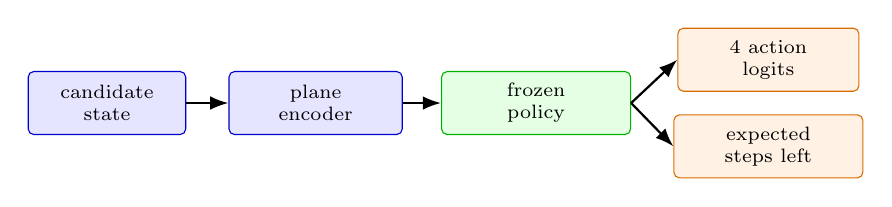
\begin{tikzpicture}[>=Latex]
    \node[draw=blue!80!black, fill=blue!10, rounded corners=2pt, align=center, minimum width=2.0cm, minimum height=0.8cm, font=\scriptsize] (state) at (0,0) {candidate\\state};
    \node[draw=blue!80!black, fill=blue!10, rounded corners=2pt, align=center, minimum width=2.2cm, minimum height=0.8cm, font=\scriptsize] (encode) at (2.65,0) {plane\\encoder};
    \node[draw=green!70!black, fill=green!10, rounded corners=2pt, align=center, minimum width=2.4cm, minimum height=0.8cm, font=\scriptsize] (policy) at (5.45,0) {frozen\\policy};
    \node[draw=orange!85!black, fill=orange!10, rounded corners=2pt, align=center, minimum width=2.3cm, minimum height=0.8cm, font=\scriptsize] (logits) at (8.4,0.55) {4 action\\logits};
    \node[draw=orange!85!black, fill=orange!10, rounded corners=2pt, align=center, minimum width=2.4cm, minimum height=0.8cm, font=\scriptsize] (value) at (8.4,-0.55) {expected\\steps left};

    \draw[->, thick] (state) -- (encode);
    \draw[->, thick] (encode) -- (policy);
    \draw[->, thick] (policy.east) -- (logits.west);
    \draw[->, thick] (policy.east) -- (value.west);
  \end{tikzpicture}
  \end{center}

  \vspace{0.4em}
  \begin{columns}[T]
    \column{0.50\textwidth}
    \textbf{Action logits}
    \begin{itemize}
      \item rank the four primitive moves;
      \item used for greedy rollout, beam expansion, and CEM sampling.
    \end{itemize}

    \column{0.50\textwidth}
    \textbf{Remaining-length head}
    \begin{itemize}
      \item predicts a discretized estimate of steps left;
      \item guides value-aware beam and best-first search.
    \end{itemize}
  \end{columns}
\end{frame}

\begin{frame}{Learned beam search loop}
  \small
  \begin{center}
  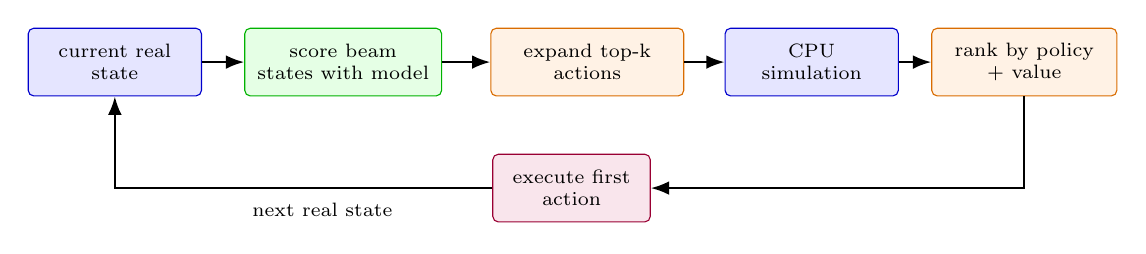
\begin{tikzpicture}[>=Latex]
    \node[draw=blue!80!black, fill=blue!10, rounded corners=2pt, align=center, minimum width=2.2cm, minimum height=0.86cm, font=\scriptsize] (root) at (0,0) {current real\\state};
    \node[draw=green!70!black, fill=green!10, rounded corners=2pt, align=center, minimum width=2.5cm, minimum height=0.86cm, font=\scriptsize] (score) at (2.9,0) {score beam\\states with model};
    \node[draw=orange!85!black, fill=orange!10, rounded corners=2pt, align=center, minimum width=2.45cm, minimum height=0.86cm, font=\scriptsize] (expand) at (6.0,0) {expand top-k\\actions};
    \node[draw=blue!80!black, fill=blue!10, rounded corners=2pt, align=center, minimum width=2.2cm, minimum height=0.86cm, font=\scriptsize] (sim) at (8.85,0) {CPU\\simulation};
    \node[draw=orange!85!black, fill=orange!10, rounded corners=2pt, align=center, minimum width=2.35cm, minimum height=0.86cm, font=\scriptsize] (rank) at (11.55,0) {rank by policy\\+ value};
    \node[draw=purple!80!black, fill=purple!10, rounded corners=2pt, align=center, minimum width=2.0cm, minimum height=0.86cm, font=\scriptsize] (act) at (5.8,-1.6) {execute first\\action};

    \draw[->, thick] (root) -- (score);
    \draw[->, thick] (score) -- (expand);
    \draw[->, thick] (expand) -- (sim);
    \draw[->, thick] (sim) -- (rank);
    \draw[->, thick] (rank.south) |- (act.east);
    \draw[->, thick] (act.west) -| (root.south);

    \node[below=2pt, font=\scriptsize]
      at ($(act.west)!0.45!(root.south |- act.west)$)
      {next real state};
  \end{tikzpicture}
  \end{center}

  \begin{itemize}
    \item Model scoring runs on GPU; candidate-state simulation and search bookkeeping run on CPU.
    \item The same state can appear in many neighboring replans.
    \item Expensive part: repeated model queries over overlapping search trees, not the four-action branching itself.
  \end{itemize}
\end{frame}

\begin{frame}{Main bottlenecks before optimization}
  \small
  \begin{columns}[T]
    \column{0.50\textwidth}
    \textbf{Where time goes}
    \begin{itemize}
      \item Beam replans after every real action.
      \item Overlapping lookahead trees repeatedly score the same states.
      \item GPU model calls are mixed with CPU search and simulation.
      \item CPU/GPU transfers are not dominant alone; redundant model work is.
    \end{itemize}

    \column{0.50\textwidth}
    \textbf{Measured signal}
    \begin{itemize}
      \item Beam without cache: 660k model-forwarded states.
      \item Beam with cache: 28.7k unique states.
      \item Same success rate: 18/68.
      \item Cache changes runtime, not solver behavior.
    \end{itemize}
  \end{columns}
\end{frame}

\begin{frame}{Reference solver: N+RGD}
  \small
  \begin{itemize}
    \item N+RGD is the official DeepMind C++ planner based on recursive graph-distance heuristics.
    \item It is the strongest reference we use: solves all Level-1 puzzles very quickly.
    \item It is not optimized for shortest plans; on puzzles solved by the learned policy, our returned path is always equal or shorter in the measured comparison.
    \item For this project, N+RGD is a reference solver and trace generator, not the system we optimize.
  \end{itemize}

  \vspace{0.7em}
  \centering
  \begin{tabular}{@{}lrrrr@{}}
    \toprule
    Method & Solved & Total time & Avg / puzzle & Solves/min \\
    \midrule
    N+RGD C++ planner & 68/68 & 6.7s & 0.10s & 607.9 \\
    Learned beam, no cache & 18/68 & 1699.6s & 25.0s & 0.64 \\
    Learned beam, cache & 18/68 & 98.2s & 1.44s & 11.0 \\
    \bottomrule
  \end{tabular}
\end{frame}

\begin{frame}{Optimization 1: prediction cache}
  \small
  \begin{columns}[T]
    \column{0.50\textwidth}
    \textbf{Target bottleneck}
    \begin{itemize}
      \item repeated model scoring for identical \((puzzle, state)\);
      \item especially strong in closed-loop beam search.
    \end{itemize}

    \textbf{Implementation}
    \begin{itemize}
      \item cache key: puzzle id + symbolic state;
      \item cache value: action log-probs and expected remaining length;
      \item no change in action selection logic.
    \end{itemize}

    \column{0.50\textwidth}
    \centering
    \resizebox{\linewidth}{!}{%
    \begin{tabular}{@{}lrrr@{}}
      \toprule
      Beam setting & Solved & Time & Relative speed \\
      \midrule
      no prediction cache & 18/68 & 1699.6s & 1.0x \\
      prediction cache & 18/68 & 98.2s & 17.3x \\
      \bottomrule
    \end{tabular}
    }

    \vspace{0.5em}
    \scriptsize
    Same solved set, fewer model forwards: 660k \(\rightarrow\) 28.7k.
  \end{columns}
\end{frame}

\begin{frame}{Optimization 2: value-guided best-first search}
  \small
  \begin{center}
  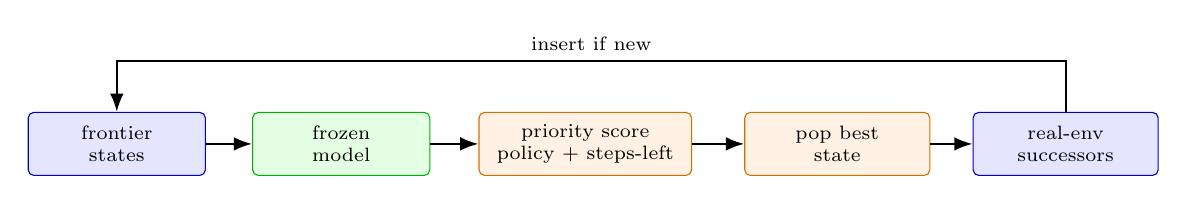
\begin{tikzpicture}[>=Latex]
    \node[draw=blue!80!black, fill=blue!10, rounded corners=2pt, align=center, minimum width=2.25cm, minimum height=0.8cm, font=\scriptsize] (frontier) at (0,0) {frontier\\states};
    \node[draw=green!70!black, fill=green!10, rounded corners=2pt, align=center, minimum width=2.25cm, minimum height=0.8cm, font=\scriptsize] (model) at (2.85,0) {frozen\\model};
    \node[draw=orange!85!black, fill=orange!10, rounded corners=2pt, align=center, minimum width=2.7cm, minimum height=0.8cm, font=\scriptsize] (score) at (5.95,0) {priority score\\policy + steps-left};
    \node[draw=orange!85!black, fill=orange!10, rounded corners=2pt, align=center, minimum width=2.35cm, minimum height=0.8cm, font=\scriptsize] (pop) at (9.15,0) {pop best\\state};
    \node[draw=blue!80!black, fill=blue!10, rounded corners=2pt, align=center, minimum width=2.35cm, minimum height=0.8cm, font=\scriptsize] (children) at (12.05,0) {real-env\\successors};

    \draw[->, thick] (frontier) -- (model);
    \draw[->, thick] (model) -- (score);
    \draw[->, thick] (score) -- (pop);
    \draw[->, thick] (pop) -- (children);
    \draw[->, thick] (children.north) -- ++(0,0.65) -| node[pos=0.25, above, font=\scriptsize] {insert if new} (frontier.north);
  \end{tikzpicture}
  \end{center}

  \begin{itemize}
    \item Beam spends a fixed budget at every depth; best-first spends the node budget on globally promising states.
    \item Priority combines policy cost and the remaining-length head.
    \item It improves search quality without changing model weights.
  \end{itemize}
\end{frame}

\begin{frame}{Best-first results}
  \small
  \centering
  \begin{tabular}{@{}lrrrr@{}}
    \toprule
    Search method & Solved & Total time & Avg / puzzle & Solves/min \\
    \midrule
    Beam + cache & 18/68 & 98.2s & 1.44s & 11.0 \\
    Best-first, budget 512 & 20/68 & 119.7s & 1.76s & 10.0 \\
    Best-first, budget 1024 & \textbf{32/68} & 199.6s & 2.94s & 9.62 \\
    \bottomrule
  \end{tabular}

  \vspace{0.7em}
  \begin{itemize}
    \item Main quality gain: 18/68 \(\rightarrow\) 32/68 on the same frozen policy.
    \item Cost increases because best-first explores more unique states.
    \item Budget 1024 is the best learned solver by success rate.
  \end{itemize}
\end{frame}

\begin{frame}{Optimization 3: GPU sampling}
  \small
  \begin{itemize}
    \item Instead of expanding a deterministic search tree, sample several policy rollouts and verify them in the real environment.
    \item This gives a speed-oriented upper bound for stochastic policy use.
    \item The current model is still the limiting factor: sampling is fast, but many sampled rollouts collapse or repeat.
  \end{itemize}

  \vspace{0.6em}
  \centering
  \begin{tabular}{@{}lrrrr@{}}
    \toprule
    Method & Solved & Total time & Avg / puzzle & Solves/min \\
    \midrule
    GPU sampling, best-of-4 & 16/68 & 48.0s & 0.71s & 20.0 \\
    Beam + cache & 18/68 & 98.2s & 1.44s & 11.0 \\
    \bottomrule
  \end{tabular}

  \vspace{0.5em}
  \scriptsize
  Fastest learned inference mode, but success rate is below beam and best-first.
\end{frame}

\begin{frame}{Optimization 4: CEM sampling}
  \small
  \begin{columns}[T]
    \column{0.50\textwidth}
    \textbf{Algorithm}
    \begin{enumerate}
      \item Sample many action sequences from the policy.
      \item Replay each sequence in the real PushWorld simulator.
      \item Keep elite rollouts by solved/progress score.
      \item Update a per-timestep action prior and resample.
    \end{enumerate}

    \column{0.50\textwidth}
    \centering
    \resizebox{\linewidth}{!}{%
    \begin{tabular}{@{}lrrrr@{}}
      \toprule
      CEM setting & Solved & Time & Avg/puzzle & Solves/min \\
      \midrule
      16x3 & 22/68 & 137s & 2.02s & 9.61 \\
      32x3 & 24/68 & 216s & 3.17s & 6.67 \\
      64x3 & 25/68 & 332s & 4.88s & 4.52 \\
      \bottomrule
    \end{tabular}
    }
  \end{columns}

  \vspace{0.6em}
  \begin{itemize}
    \item CEM improves over simple sampling, but runtime grows quickly.
    \item It is an exploratory alternative, not the final best tradeoff.
  \end{itemize}
\end{frame}

\begin{frame}{Optimization 5: GPU-resident particle rollout}
  \small
  \begin{itemize}
    \item Goal: move candidate rollout dynamics to GPU instead of calling the Python simulator for every candidate.
    \item Exact backend: one fused Triton kernel for PushWorld transition.
    \item Approximate backend: point-object dynamics, faster but not always faithful.
    \item Particle count means how many candidate trajectories are simulated in parallel for one puzzle.
    \item Result: exact GPU transition works, but end-to-end search is still dominated by policy refresh and verification.
  \end{itemize}

  \vspace{0.45em}
  \centering
  \resizebox{0.86\textwidth}{!}{%
  \begin{tabular}{@{}lrrl@{}}
    \toprule
    Variant & Scale & Smoke result & Verdict \\
    \midrule
    Beam + cache & 5 puzzles & 1/5 in 7.5s & comparison run \\
    Exact Triton particles & 128 particles & 1/5 in 68s & too slow/weak \\
    Exact Triton particles & 512 particles & 2/5 in 238s & more success, too slow \\
    Approx dynamics & 128 particles & false positives & needs exact replay filter \\
    \bottomrule
  \end{tabular}
  }

\end{frame}

\begin{frame}{Ranker experiment}
  \small
  \begin{itemize}
    \item We tested a hand-written ranker term inside best-first priority.
    \item No additional model was trained: priority used policy cost, remaining-length estimate, goal distance, and achieved-goal bonus.
    \item This was a cheap proxy for learned state ranking.
    \item Result: no measurable gain over baseline best-first 1024.
  \end{itemize}

  \vspace{0.6em}
  \centering
  \begin{tabular}{@{}lrrrr@{}}
    \toprule
    Search priority & Solved & Total time & Avg / puzzle & Solves/min \\
    \midrule
    policy + remaining length & 32/68 & 199.6s & 2.94s & 9.62 \\
    + goal-distance ranker term & 32/68 & 199.8s & 2.94s & 9.61 \\
    \bottomrule
  \end{tabular}
\end{frame}

\begin{frame}{Final comparison}
  \small
  \centering
  \resizebox{\textwidth}{!}{%
  \begin{tabular}{@{}lrrrrl@{}}
    \toprule
    Method & Solved & Time & Avg / puzzle & Solves/min & Role \\
    \midrule
    N+RGD planner & 68/68 & 6.7s & 0.10s & 607.9 & reference solver \\
    Beam, no cache & 18/68 & 1699.6s & 25.0s & 0.64 & bottleneck baseline \\
    GPU sampling & 16/68 & \textbf{48.0s} & \textbf{0.71s} & \textbf{20.0} & fastest learned mode \\
    Beam + cache & 18/68 & 98.2s & 1.44s & 11.0 & cached baseline \\
    CEM 16x3 & 22/68 & 137.3s & 2.02s & 9.61 & stochastic search \\
    Best-first 1024 & \textbf{32/68} & 199.6s & 2.94s & 9.62 & best learned success \\
    \bottomrule
  \end{tabular}
  }

  \vspace{0.65em}
  \begin{itemize}
    \item Final choice for quality: \textbf{prediction cache + best-first 1024}.
    \item Final choice for raw speed: GPU sampling, but with lower success.
  \end{itemize}
\end{frame}

\begin{frame}{Future work}
  \small
  \begin{enumerate}
    \item \textbf{Learned ranker for search nodes.}\\
    Train a lightweight ranker on states expanded by best-first: solution-path states as positives, dead/repeated frontier states as negatives. Use it to reduce node budget without losing solved puzzles.

    \item \textbf{Adaptive search budget.}\\
    Start with cheap sampling or BF-512, then escalate only when confidence/progress is low. This targets better average time per puzzle instead of one fixed budget for all maps.

    \item \textbf{Proposal + verification split.}\\
    Use fast approximate or GPU proposals only to generate candidate action sequences, then always verify the final path in exact PushWorld dynamics.
  \end{enumerate}
\end{frame}

\begin{frame}{Code}
  \centering
  \begin{columns}[c]
    \column{0.50\textwidth}
    \centering
    \qrcode[height=0.48\textheight]{https://github.com/eivankin/pushworld}

    \vspace{0.5em}
    \small
    \href{https://github.com/eivankin/pushworld}{github.com/eivankin/pushworld}

    \column{0.50\textwidth}
    \centering
    \qrcode[height=0.48\textheight]{https://github.com/adam-suliman/pushworld}

    \vspace{0.5em}
    \small
    \href{https://github.com/adam-suliman/pushworld}{github.com/adam-suliman/pushworld}
  \end{columns}
\end{frame}

\end{document}
